\documentclass[conference]{IEEEtran}
% correct bad hyphenation here
\hyphenation{op-tical net-works semi-conduc-tor}

\usepackage{hyperref, textcomp, pgfplots, url, cite}
\pgfplotsset{width=7cm,compat=1.9}

\begin{document}
\title{Poster: Obliv-C Language as a Tool for \\Scalable Privacy-Preserving Data Analysis}

\author{\IEEEauthorblockN{Samuel Havron
\IEEEauthorblockA{
Undergraduate Researcher\\ \emph{University of Virginia}\\ % necessary to include title? 
\href{mailto:havron@virginia.edu}{havron@virginia.edu}\\
}
}
}

\maketitle

% IEEE POSTER REQUIREMENTS:
%Submit an abstract no longer than two pages describing the work. The abstract title should begin with the keyword "Poster:". Include all authors with contact information and institutional affiliation in your abstract.
%Your abstract should not exceed the two page limit; non-conforming submissions will not be considered for review.
%If accepted, at least one author must be registered and a final version of the poster abstract submitted by Friday, May 13, 2016.

\begin{abstract}
A \emph{Secure multi-party computation} (MPC) is a protocol which allows for two or more parties to compute a function on sensitive input data provided by each party, without revealing anything about the inputs (other than what can be inferred from the revealed output result). 
Using the OblivC language, researchers can develop their own application-specific
MPCs and quickly deploy them for use in scalable privacy-preserving data analysis.
A demonstration of the scalability and performance of OblivC and a discussion of
related work highlights the utility of the language for researchers who have little
to no experience in cryptographic protocols. 
\end{abstract}

\section{Introduction}
Most current implementations of MPC work by executing instructions in a \emph{data-oblivious} manner, where the control flow of the program is independent of the 
inputs provided by each party and the program executes without any 
knowledge of the cleartext data it is operating on.
This effectively creates a black box, such that semi-honest adversaries cannot gain addition insight about the source data, receiving only the computated results.
Many researchers and social scientists need MPCs in order to analyze datasets that are 
both large and sensitive, and they often need to rely on using an underlying secure computation software framework to execute such MPCs.
However, the software framework chosen for developing an application can greatly
affect the researcher's ability to use and modify protocols to suit their individual needs.
The titular language of this paper is one such framework that will be discussed in depth.

Frameworks currently available can typically be categorized as either very low-level, requiring the researcher to be adept in cryptography and circuit structures, or very high-level, limiting the ability of the researcher to directly experiment with protocols 
and extend the underlying design of the tools available.
A third category of frameworks, "domain-specific languages", are more mature than
the low-level programming libraries, but less mature than high-level libraries and tools\cite{cryptoeprint:2015:1039}.
They are suitable for allowing a researcher the freedom to modify and develop
their own protocols without concern of low-level details or high-level constraints.

One such "domain-specific language" is OblivC, a new programming language 
which is designed to make it simple for anyone to write software which provides 
secure protocols for analyzing data and fitting individual requirements 
for a particular project\cite{cryptoeprint:2015:1153}. The language is compiled and built 
on top of the standard C language, allowing for developers to 
integrate C tools with OblivC seamlessly (it is called "domain-specific" for 
this reason: OblivC integrates with the C programming language and its standard libraries).
OblivC implements secure MPC through optimizations of Yao's garbled circuit protocol for use with semi-honest adversaries.
Using this language to write applications that can analyze large, privacy-preserving
datasets is presented in a comprehensive tutorial online\cite{tutorial:oblivc}, and results of building one such application for linear regression analysis 
are shown in Preliminary Results.

\section{Approach}
OblivC is a programming language which allows an application developer to
quickly implement scalable, secure MPC protocols, using the language’s 
Application Programming Interface ("API", included in the standard OblivC
library) or writing specific functionality by extending the language's existing library as
well as experimenting with the implementation of library protocols.
The goal of using OblivC as a framework for secure computation is to demonstrate 
its performance capabilities and ease of use to developers whom have little 
knowledge of cryptography or circuit structures, but would greatly benefit from 
using secure MPCs to carry out privacy-preserving dataset analysis (perhaps for
social science research).

% is approach too similar to introduction? I feel I am repeating my words.
While the preliminary results of testing OblivC's capabilities are below, the process for
a developer to start using OblivC was also written as a comprehensive tutorial online\cite{tutorial:oblivc},
including a walkthrough of writing an OblivC program and linking it appropriately 
to C programs.
Installing the compiler and libraries are also documented, in addition to a documentation
of the API used in the walkthrough.

\section{Preliminary Results/Discussion}
A linear regression program was developed to test the scalability and speed of OblivC as a tool for implementing MPC programs. 
Testing was done using c4.large \emph{Elastic Compute Cloud} (EC2) nodes from \emph{Amazon Web Services} (AWS)\cite{aws:ec2}, which feature 
high frequency Intel Xeon E5-2666 v3 (Haswell) processors optimized specifically for EC2,
two vCPUs, and 3.75 GiB of DRAM.
Two c4.large instances were launched and connected through 
OblivC's API for TCP/IP connections. The instances were both located in the same cloud
cluster in Oregon; exploring network latency issues with secure MPCs is also of interest.

One node instance provided independent ($x$) data points, while the other provided dependent ($y$) data points; data points used were 32-bit integers, using fixed-point 
mathematics to convert raw data values into scaled integers, as 
OblivC does not currently support floating point numbers.
The time needed to execute the MPC between instances appears to scale linearly 
with the size of the data input, as seen in Figure 1; 100K data points finished execution in 12.7 minutes 
on average, 500K completed in 63.7 minutes, and 1 million data points finished execution 
in just over 127 minutes on average.

Artificial data was generated for testing the scalability of input size, and
considerations to automated data match-ups between two separate datasets were not
implemented; the artifical data was presumed to already be matched and sorted properly.
\begin{figure}[!t]
\centering
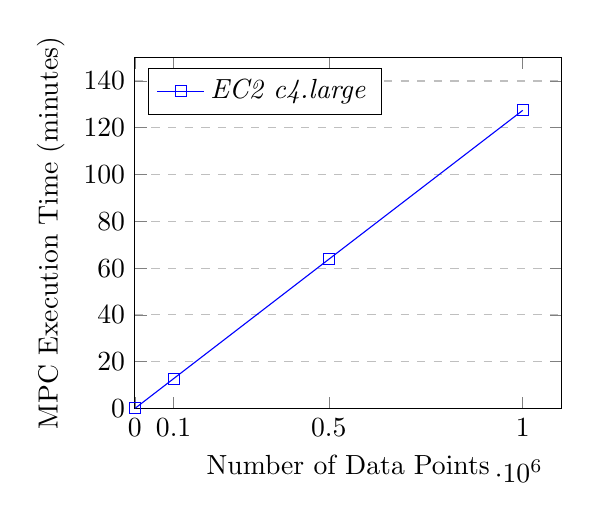
\begin{tikzpicture}
\begin{axis}[
    %title={Performance of MPC linear regression analysis},
    xlabel={Number of Data Points},
    ylabel={MPC Execution Time (minutes)},
    xmin=0, xmax=1100000,
    ymin=0, ymax=150,
    xtick={0,100000,500000,1000000},
    ytick={0,20,40,60,80,100,120,140},
    legend pos=north west,
    ymajorgrids=true,
    grid style=dashed,
]
\addplot[
    color=blue,
    mark=square,
    ]
    coordinates {
    (1000,0.1088522)(100000,12.74658383)(500000,63.765116616)(1000000,127.42427975)
    };
    \legend{\emph{EC2 c4.large}}
 
\end{axis}
\end{tikzpicture}
\caption{Performance of MPC linear regression analysis.}
\label{xy_plot}
\end{figure}
To provide a clear example of the utility of OblivC for analyzing sensitive datasets, additional data for computation was obtained from the public 
New York State Department of Health dataset of Hospital Inpatient Discharges from 2011\cite{healthdata:ny}. 
Comparisons between fields such as "Length of Days stayed" and "Total Costs" over approximately 2.6 million data points are currently being tested.
This dataset is particularly amenable to analysis, as all data is already matched properly and each data value is a comparable number.
However, using OblivC's API for private set intersection and ORAM access with a unique identifier (such as SSN) is also being investigated so as to provide an application which can match all datapoints from two separate datasets which are tied to a common identifier.

\section{Related Work}
A similar approach in taking distinct federal datasets and comparing them is seen in
Dan Bogdanov \emph{et al.}, where correlations between working hours and failure to
graduate on time in Estonia was investigated, matching over 10 million 
tax records and 500K education records\cite{cryptoeprint:2015:1159}.
Undertaking such a massive task used the researchers' own framework for secure
computation, \emph{ShareMind}, a database and analytics system implemented at a higher-level than OblivC to provide secure MPCs. 
% related work section needs to be expanded? or is it sufficient?
% what makes Obliv-C distinct from ShareMind, other than the relatively high-level
% of the latter? (it also has an open-source SDK with a C-like language.
\section{Conclusion}
The OblivC language is well-suited to developing application-specific functionality for scalable, sensitive data analysis between two or more parties.
Researchers who are not experts in cryptography can easily develop secure protocols
using OblivC for their work, without needing to experiment with basic primitives
and other low level aspects of the language's implementation of secure computation.
Future work may include a closer examination of automatic data-matching between
separate datasets, improving fixed-point integer conversion for decimal data values,
and conducting a formal comparison of OblivC's performance in scalable
data computations for statistical analysis with similar software tools,
such as Rmind\cite{eprint:BKLS14}.

% trigger a \newpage just before the given reference
% number - used to balance the columns on the last page
%\IEEEtriggeratref{8}
% The "triggered" command can be changed if desired:
%\IEEEtriggercmd{\enlargethispage{-5in}}

% references section
\begin{thebibliography}{1}

\bibitem{aws:ec2}
  \url{https://aws.amazon.com/ec2/instance-types/}.

\bibitem{healthdata:ny}
  \url{https://health.data.ny.gov/}.

\bibitem{tutorial:oblivc}
  \url{http://samuelhavron.github.io/obliv-c/}

\bibitem{cryptoeprint:2015:1039}
    David W. Archer and Dan Bogdanov and Benny Pinkas and Pille Pullonen,
    \emph{Maturity and Performance of Programmable Secure Computation},
    Cryptology ePrint Archive, Report 2015/1039,
    2015,
    \url{http://eprint.iacr.org/}

\bibitem{cryptoeprint:2015:1159}
    Dan Bogdanov, Liina Kamm, Baldur Kubo, Reimo Rebane, Ville Sokk, Riivo Talviste,
    \emph{Students and Taxes: a Privacy-Preserving Social Study Using Secure Computation},
    Cryptology ePrint Archive, Report 2015/1159,
    2015,
    \url{http://eprint.iacr.org/}.

\bibitem{eprint:BKLS14}
    Dan Bogdanov and Liina Kamm and Sven Laur and Ville Sokk,
    \emph{Rmind: a tool for cryptographically secure statistical analysis},
    Cryptology ePrint Archive, Report 2014/512,
    2014,
    \url{http://eprint.iacr.org/}.
% not being used ... for now.
%\bibitem{UT:Kamm15}
 % Liina Kamm, 
 % \emph{Privacy-preserving statistical analysis using secure multi-party computation},
 % University of Tartu, 2015,
 % \url{http://hdl.handle.net/10062/45343}.

\bibitem{cryptoeprint:2015:1153}
  Samee Zahur and David Evans, \emph{Obliv-C: A Language for Extensible 
  Data-Oblivious Computation}, Cryptology ePrint Archive, 
  Report 2015/1153, 2015, 
  \url{http://eprint.iacr.org/}.

\end{thebibliography}
\end{document}
